\documentclass[compress,red]{beamer}
\mode<presentation>

\usetheme{Warsaw}

%\hypersetup{pdfpagemode=FullScreen}

\useoutertheme[subsection=false]{smoothbars}
\useinnertheme{rectangles}
\usepackage[square, numbers, comma, sort&compress]{natbib}  % Use the "Natbib" style for the references in the Bibliography

%\setbeamertemplate{footline}[text line]{} 

%\usepackage{beamerthemesplit}
\usepackage{graphicx}
\usepackage{amsmath}
\usepackage{listings}
\usepackage{alltt}


\title{Complete System Testing}
\author[Sanath Kumar Ramesh]
{
	\textbf{Sanath Kumar Ramesh\ \\}
	{\ \\ \small{CSE 218}\ \\ \ \\ \ \\}
}


\date[]{ May 25, 2011}

\begin{document}

\frame{\titlepage}


\frame
{
	\frametitle{Today's Papers}
	\begin{enumerate}
	
	 \item \textbf{Automatic system testing of programs without test oracles}, Christian Murphy, Kuang Shen, and Gail Kaiser.

	\item \textbf{Automating System Tests Using Declarative Virtual Machines}, van der Burg, S.; Dolstra, E.
	
	\item \textbf{A formal analysis of requirements-based testing}, Charles Pecheur, Franco Raimondi, and Guillaume Brat.
	\end{enumerate}
}

\section{Auto Metamorphisis Testing}
\frame{
	\begin{center}
	{ \Large { \textsc{Automatic System Testing of Programs without Test Oracles} } }\\
	\ \\
	Christian Murphy, Kuang Shen, Gail Kaiser \\
	Columbia University
	\end{center}
}

\frame
{
	\frametitle{Problem Landscape}
	\pause
	\textbf{Metamorphic Testing} -
	\pause System testing where test oracles are not applicable.. \\	
	\pause \textbf{What are test oracles?} - \pause An oracle is a mechanism for determining whether the program has passed or failed a test. \\
		
	\pause \textbf{When are test oracles not applicable?}
	\pause
	\begin{itemize}
		\item Input, Output cannot be clearly defined.. 
		\pause
		Example:
		\begin{itemize}
			\item What is the input to an airplane autopilot system??
			\pause
			\item What is its output??
			\pause
			\item A Simpler example..\pause Input to a program calculating PI
			\pause
			\item Output????? 
		\end{itemize}
		\pause
		\item Generally, Scientific calculations, optimizations, machine learning etc fall in this category
	\end{itemize}
}

\frame
{

	\frametitle{Metamorphic Testing - How is it done?}
	\begin{itemize}
		\item Simple inputs and outputs to the system are identified
		\pause
		\item System is first tested with them
		\pause
		\item Modify existing test case input to produce new test case such that new output can be predicted from the existing output
		if $x$ is the old input, $f(x)$ is old output, then create new input $x'$ from $x$ such that $f(x')$ can be predicted from $f(x)$
	\end{itemize}
}

\frame
{
	\frametitle{But..}
	\begin{itemize}
		\item Very hard to manually enerate new inputs..
		\pause
		\item Even harder to validate the new output
		\pause
		\item
		They are even called ``Non-Testable'' programs
		\item Alternative??
		\pause
		\begin{itemize}
			\item[*] \textbf{Pseudo-Oracle} \\
				Make multiple implementations of same program with different algorithms and validate output..!! 
			\item[*] \textbf{Automated Metamorphic System Testing(Paper's proposal)} \\
				Automate the process of creating various inputs, running the test and validating the output
		\end{itemize}
	\end{itemize}
}

\frame
{
	\frametitle{Automatic Metamorphic System Testing Framework}
	\begin{center}
	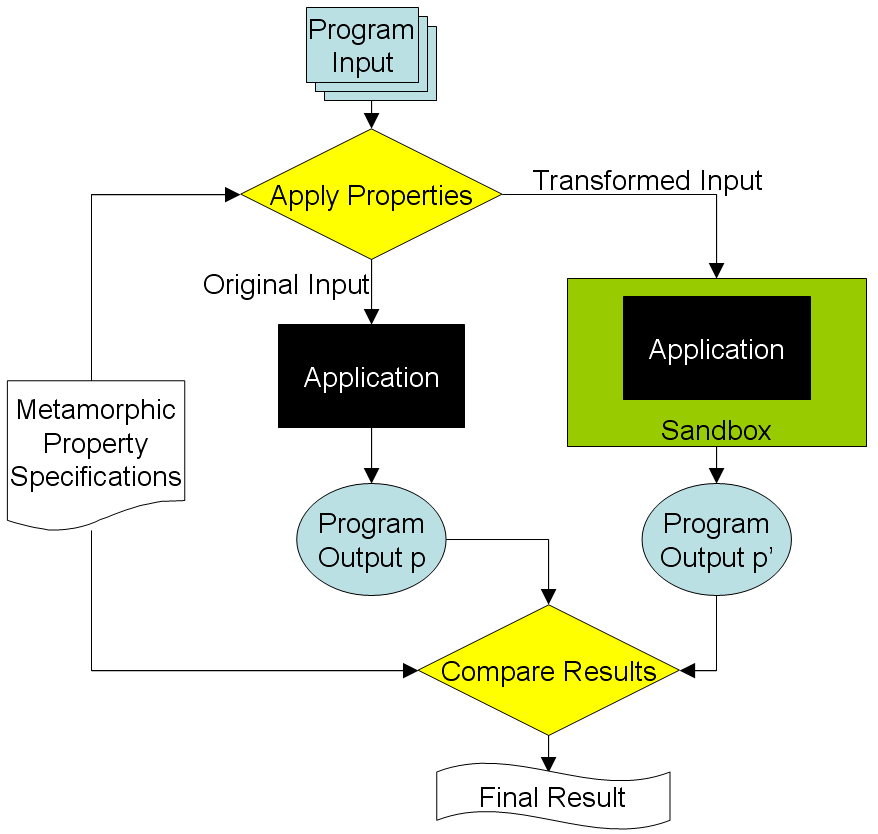
\includegraphics[scale=0.25]{amst-framework.png}
	\end{center}
}

\frame
{
	\frametitle{Framework Description}
	\textbf{Input Transformations}
	\begin{itemize}
		\item XML file specifies the transformation type
		\pause
		\item[] 6 transformations are implemented:
				\begin{enumerate}
					\item Adding a constant to numerical values
					\item Multiplying numerical values by a constant
					\item Permuting the order of input data
					\item Reversing the order of input data
					\item Removing part of data
					\item Adding additional data
				\end{enumerate}
	\end{itemize}
}


\frame
{
	\frametitle{Framework Description}
	\textbf{Metamorphic Property Specification XML}
	\begin{center}
	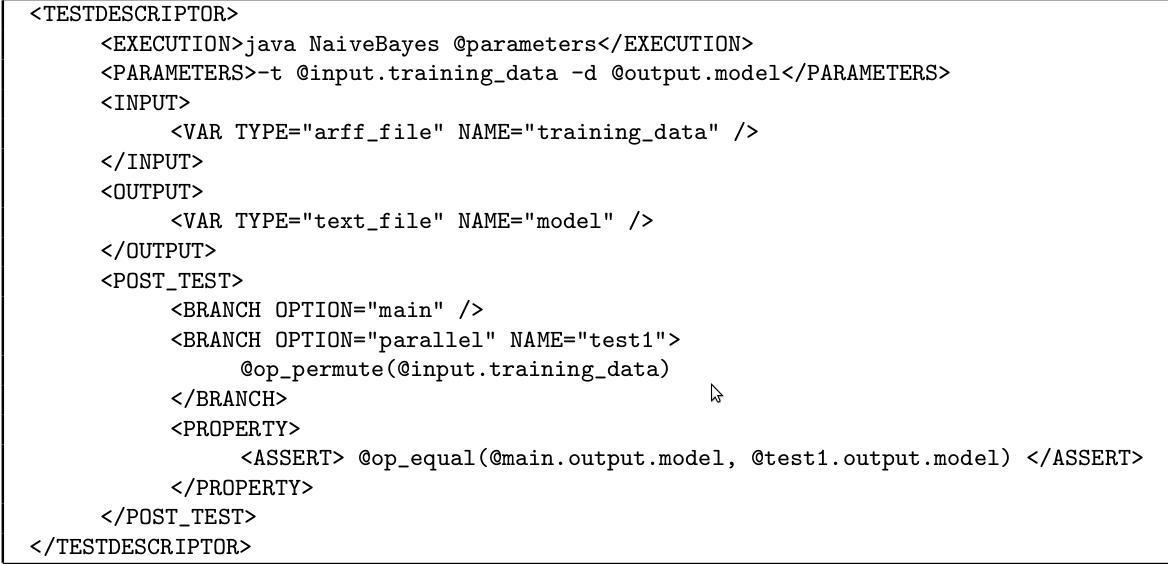
\includegraphics[scale=0.25]{amst-input-xml.png}
	\end{center}

}


\frame
{
	\frametitle{Framework Description}
	\textbf{Program Execution}
	\begin{itemize}
		\pause
		\item Copy all files needed for application execution
		\pause	
		\item Initialize application inside a sandbox - Amsterdam + ``pod'' (virtualization layer)
		\pause
		\item Execute either in 
			\begin{itemize}
				\pause
				\item Production Environment - Run by end-user after deployment
					\begin{itemize}
						\item Invoke sanboxed application and ``functional'' app parallely
					\end{itemize}
				\pause
				\item Development Environment - Pre-release testing
					\begin{itemize}
						\item Can disable parallel execution \& Sandboxing
						\item Trace dump enable
					\end{itemize}
			\end{itemize}
		\pause
		\item If test fails, Pop-up message or write to file
	\end{itemize}
}

\frame
{
	\frametitle{Framework Description}
	\textbf{Output Comparison}
	\begin{itemize}
		\item[] Output Match $\implies$ No fault in program
		\item[] Output Mismatch $\implies$ Fault Detected !!
			\begin{itemize}
				\pause
				\item[*] Exact mismatch
				\pause
				\item[*] Approximate Mismatch - 
				\item[] Ex: Floating Point results
				\item[] Value of $sine(x)$ and $sine(x + 2\pi)$ should be same. But the precision depends on value of $\pi$ used in the program.
				\pause
				\item[]
				\item[] Use \textit{Heuristic Metamorphic Testing} - Upto 2\% mismatch allowed
			\end{itemize}
	\end{itemize}
}



\frame
{
	\frametitle{Empirical Sutdies}
	Evaluated on 3 machine learning applications from Weka 3.5.8 toolkit (Java)
	\begin{itemize}
		\item \textbf{Support Vector Machines} - Supervised classification
		\item \textbf{C4.5} - Decision tree builder
		\item \textbf{MartiRank} - Ranking algorithm
		\item \textbf{PAYL} - Network packets anomoly based intrusion detection system
	\end{itemize}

}

\frame
{
	\frametitle{Empirical Sutdies}
	\textbf{Experiment Methodoly}
	\begin{itemize}
		\item Insert random mutation in source code
		\item Determine if mutation can be detected by the testing suite
	\end{itemize}
\ \\ \ \\ 	
	Three mutant types used:
	\begin{itemize}
		\item Flip comparison operators: $=$  becomes $\neq$
		\item Flip mathematical operators: $*$ become $\div$
		\item Off-by-one error: adjust loop variable, array indices etc by one
	\end{itemize}

}

\frame
{
	\frametitle{Results}
	\begin{center}
	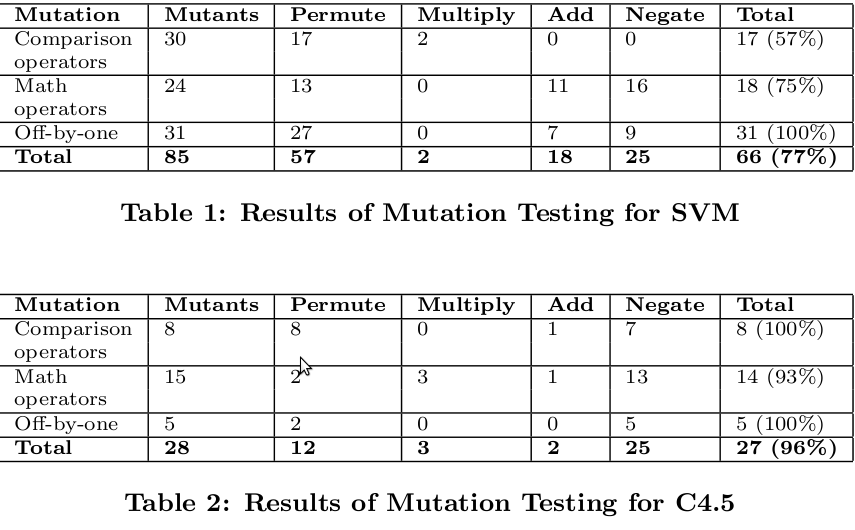
\includegraphics[scale=0.3]{amst-table1.png}
	\end{center}

}

\frame
{
	\frametitle{Results}
	\begin{center}
	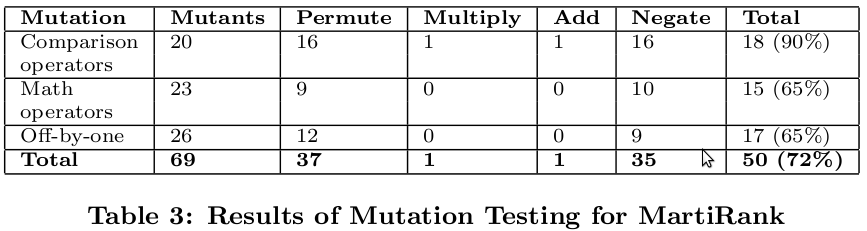
\includegraphics[scale=0.3]{amst-table2.png}
	\end{center}

	\textbf{For PAYL:} \\
	 - Detected 2 of 40 mutants !! \\
	 - Reason: PAYL bothers about distribution of data. Input metamorphosis altered content and ordering only, not distribution. 
}

\frame
{
	\frametitle{Performance}
	Quad-core 3GHz CPU running Ubuntu \\
	- 400ms lag in \textit{application startup} for 10MB input file \\  
	- ``Functional Application'' and ``Sanboxed Application'' ran on different cores without measurable lag to user

}

\frame
{
	\frametitle{Snake Oil}
	\begin{itemize}
		\item Can't work with Databases and Network 
		\item Can't work for applications requiring user response 
		\item Fault Localization not possible
		\item Can't work for binary input/output 
		\item No false +ve rate mentioned in paper
	\end{itemize}
}

\section{Test with Declarative VMs}
\frame{
  
	\begin{center}
	{ \Large { \textsc{Automating System Tests Using Declarative Virtual Machines} } }\\
	\ \\
	Sander van der Burg, Eelco Dolstra \\
	Delft University of Technology, The Netherlands
	\end{center}
}

\frame
{
	\frametitle{Problem Landscape}
	\begin{itemize}
		\pause
		\item To run regression suite on entire application
		\pause
		\item Heavy dependency between modules
		\pause
		\item Application requires specific \textit{system environment} \\
			  For example: 
			  \begin{itemize}
			  	\pause
			  	\item \textbf{OpenSSH} requires super-user privileges to run; needs multiple user accounts
			  	\pause
				\item \textbf{Quake 3 Arena} needs networked machines to start a client and server
				\pause
				\item \textbf{Transmission} requires a host behind NAT with UPnP-IGD protocol enabled router
			  \end{itemize}
	\end{itemize}
	\ \\
	\pause
	 \center { \textsc{ how to AUTOMATICALLY RUN regression test? } }
}

\frame
{
	\frametitle{Solution}
	\begin{center} \Large{ \textsc{NixOS} }  \end{center}
	Build and instantiate Virtual Machine and run application inside it
}
\frame
{
	\frametitle{What is NixOS?}
	\begin{itemize}
		\pause
		\item OS built out of a Purely functional Package Manager - NIX
		\pause
		\item Makefile-like script to build and run a Linux OS
		\pause
		\item Can specify packages to be installed inside the built OS
		\pause
		\item Will automatically dependencies and build them
		\pause
		\item Supports multiple builds simultaneously with different configurations
		\pause
		\item Runs NixOS on QEMU/KVM Hardware Emulator
	\end{itemize}
}

\begin{frame}[fragile]

	\frametitle{Nix Expression Script}
	\begin{verbatim}
		derivation {
		  name = "foo";
		  builder = "${bash}/bin/sh";
		  args = [ "-c" "echo Hello $who > $out" ];
		  who = "world";
		}
	\end{verbatim}

Output: ``Hello world'' will be written into /nix/store/lw1e3or1p45n2-foo
\end{frame}

\frame
{
	\frametitle{Nix Expression Script}
	To build Apache: \texttt{nix-build pkgs.nix -A httpd}
	\begin{center}
	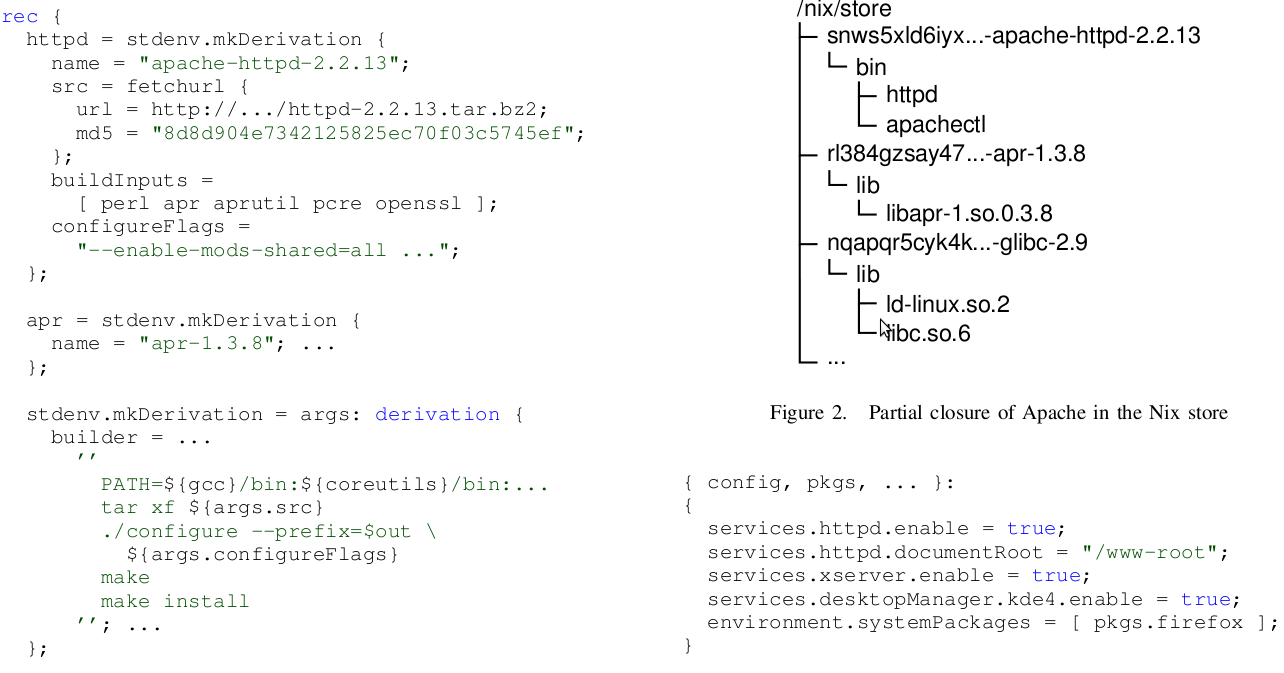
\includegraphics[scale=0.25]{vm-apache.png}
	\end{center}

}

\frame
{
	\frametitle{Building NixOS from scratch}
	\small{\texttt{nix-build /etc/nixos/nixos -A config.build.system.toplevel}}
	\pause
	
}

\frame
{
	\frametitle{Testing OpenSSH}
	\texttt{\$ nix-build openssh.nix -A vm} \\
	\texttt{\$ ./result/bin/run-vm}
	\begin{center}
	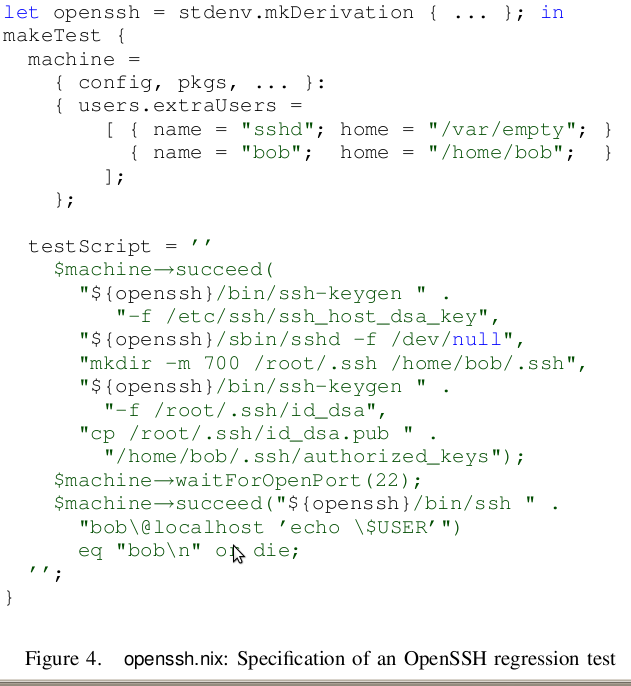
\includegraphics[scale=0.25]{vm-openssh.png}
	\end{center}
}

\frame
{
	\frametitle{Distributed Tests - For Transmission}
	Network Specification 
	\begin{center}
	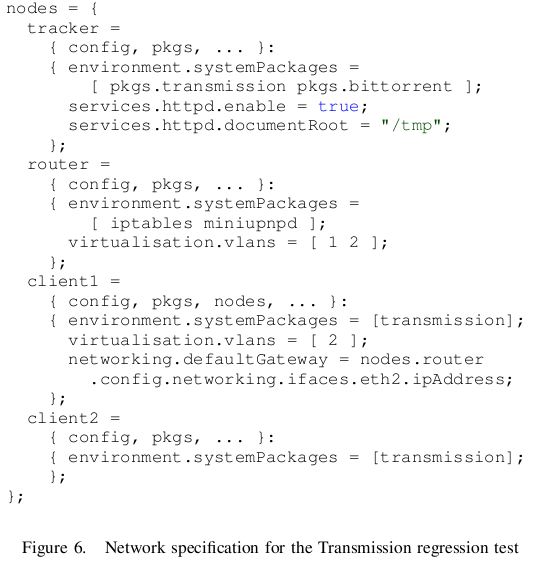
\includegraphics[scale=0.3]{vm-transmission-nix.png}
	\end{center}
}

\frame
{
	\frametitle{Distributed Tests - For Transmission}
	 Test Script 
	\begin{center}
	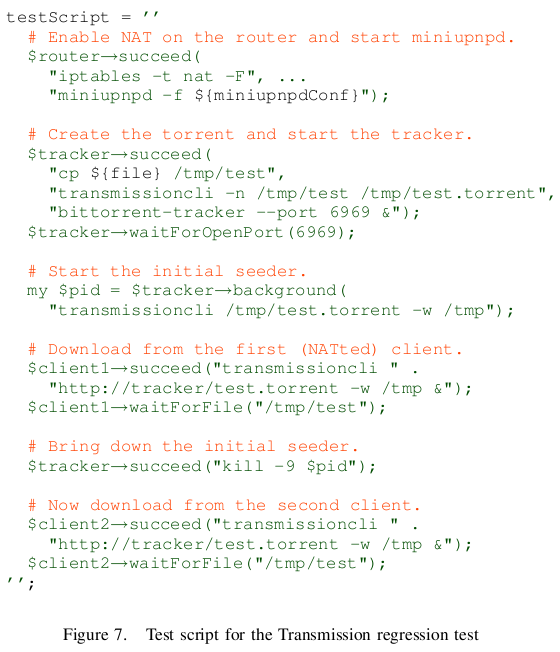
\includegraphics[scale=0.3]{vm-transmission-perl.png}
	\end{center}
}

\frame
{
	\frametitle{Evaluation}
	Coverage:- \\
	\pause
	Apache + SVN + Linux Kernel was instrumented: \\
	\pause
	Run client on one VM, server on another VM; Evaluate coverage together for both!!
	\pause
	\begin{center}
	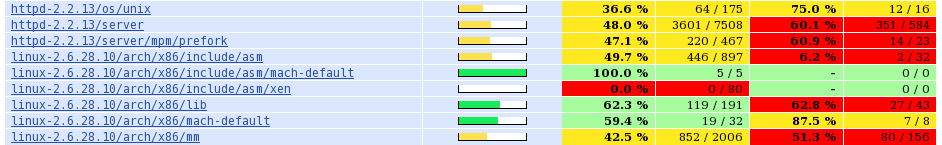
\includegraphics[scale=0.35]{vm-coverage.png}
	\end{center}
}

\frame
{
	\frametitle{Evaluation}
	Resource Consumption on 4-core Intel Core i5 with 6GiB RAM
	\begin{center}
	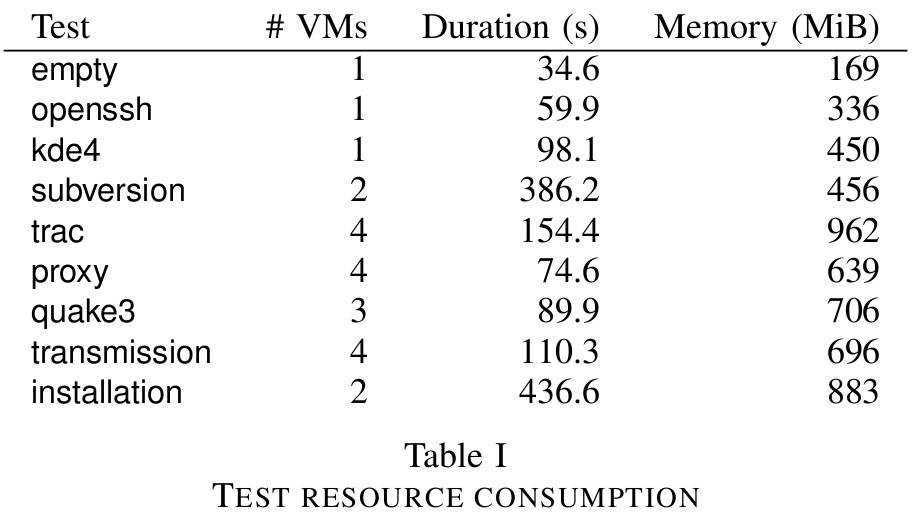
\includegraphics[scale=0.26]{vm-resource.png}
	\end{center}
	\pause
	$>>>$ Fast enough to do \textbf{continuous builds} $<<<$
}

\frame
{
	\frametitle{Snake Oil}
	\pause
	Seems like an ultimate solution to system testing..
	\pause
	NO !!
	\begin{itemize}
		\pause
		\item GUI testing not possible
		\pause
		\item Only for Linux applications
		\pause
		\item Not for scalability testing - Can't spawn 1000 VMs..!!
	\end{itemize}
}

\section{Formal Analysis of Req. Test}
\frame{
  
	\begin{center}
	{ \Large { \textsc{A Formal Analysis of Requirements-Based Testing} } }\\
	\ \\
	Charles Pecheur,, Franco Raimondi, Guillaume Brat\\
	\end{center}
}

\frame
{
	\frametitle{Problem Landscape}
	\begin{itemize}
		\pause
		\item Requirements-based Testing - generate test cases from requirements
		\pause
		\item Difficult because requirements are in natural language
		\pause
		\item Very critical for avionics - Ex: MARS Rovers 
		\pause
		\item Model checkers are slow - Massive state space
		\pause
		\item Requirements are temporal - Ex: if the rover is moving, then all instruments are stored
	\end{itemize}
}

\frame
{
	\frametitle{Solution}
	\begin{itemize}
		\pause
		\item Express requirements in Linear Temporal Logic 
		\pause
		\item FLIP - A formalism prove that an execution path $\pi$ is an adequate test case for a formula $\phi$ and an atom $a$ appearing in the formula. 
	\end{itemize}
}

\frame
{
	\frametitle{Modified Condition/Decision Coverage metric}
	\pause
	MC/DC metric is critical for avionics software. \\
	\pause
	For test suite to achieve MC/DC coverage:
	\pause
	\begin{enumerate}
		\item Every basic condition in any decision has been taken on all possible outcomes at least one
		\item Each basic condition has been shown to \textbf{independently} affect the decision's outcome.
	\end{enumerate}

	\pause
	\begin{center}
	\begin{tabular}{|c c|c|}
	\hline
		a & b & a $\lor$ b \\ \hline
		T & F & T \\ \hline
		F & T & T \\ \hline
		F & F & F \\ \hline
	\end{tabular}
	\end{center}

	- Can't work when conditions are coupled - Ex: $(a \land b) \lor (\lnot a \land c))$
}

\frame
{
	\frametitle{Implementat Details}
	\begin{itemize}
		\pause
		\item Rules are implemented in \textit{Maude}
		\pause
		\item Verified with NuSMV and Maude module
		\pause
		\item Restricted to \textit{linear formulae} for requirements
	\end{itemize}
}

\begin{frame}[fragile]

	\frametitle{References}
\small{
	1. Christian Murphy, Kuang Shen, and Gail Kaiser. 2009. Automatic system testing of programs without test oracles. In Proceedings of the eighteenth international symposium on Software testing and analysis (ISSTA '09). ACM, New York, NY, USA, 189-200. DOI=10.1145/1572272.1572295  \\
\ \\
	2. van der Burg, S.; Dolstra, E.; , "Automating System Tests Using Declarative Virtual Machines," Software Reliability Engineering (ISSRE), 2010 IEEE 21st International Symposium on , vol., no., pp.181-190, 1-4 Nov. 2010 doi: 10.1109/ISSRE.2010.34 \\ 
\ \\
	3. Charles Pecheur, Franco Raimondi, and Guillaume Brat. 2009. A formal analysis of requirements-based testing. In Proceedings of the eighteenth international symposium on Software testing and analysis (ISSTA '09). ACM, New York, NY, USA, 47-56. DOI=10.1145/1572272.1572279 \\
}
\end{frame}

\frame
{
	\begin{center}
		\Large{Thank you !!}
	\end{center}
	
}
\end{document}
